\documentclass[final]{beamer}


\usepackage[scale=1.24]{beamerposter} % Use the beamerposter package for laying out the poster
\usetheme{confposter} % Use the confposter theme supplied with this template

% Enhanced color scheme - professional and visually appealing
\definecolor{mainblue}{RGB}{41, 128, 185} % Professional blue for main elements
\definecolor{secondaryblue}{RGB}{52, 152, 219} % Lighter blue for secondary elements
\definecolor{accent}{RGB}{155, 89, 182} % Purple accent for highlights
\definecolor{highlight}{RGB}{27, 133, 69} % Darker green highlight for important points
\definecolor{darkgray}{RGB}{52, 73, 94} % Dark gray for main text
\definecolor{lightgray}{RGB}{236, 240, 241} % Light gray for backgrounds
\definecolor{warmorange}{RGB}{140, 70, 20} % Warm orange for attention points
\definecolor{softred}{RGB}{231, 76, 60} % Softer red that's easier on the eyes
\definecolor{teal}{RGB}{15, 120, 100} % Teal for alternative highlighting
\definecolor{goldenrod}{RGB}{243, 156, 18} % Golden color for contrastive learning

\definecolor{modernhighlight}{RGB}{20, 110, 70}
\newcommand{\hlmodern}[1]{\textcolor{modernhighlight}{#1}}


% Midnight blue – deep and elegant
\definecolor{midnight}{RGB}{25, 32, 72}

% Deep plum – moody and refined
\definecolor{deepplum}{RGB}{72, 0, 72}

% Forest black – nearly black with a hint of green
\definecolor{forestblack}{RGB}{10, 30, 25}

% Graphite – smooth dark gray for text or UI blocks
\definecolor{graphite}{RGB}{33, 37, 41}

% Steel blue – dark and techy
\definecolor{steelblue}{RGB}{54, 69, 79}

% Charred red – deep, rich red without being too bright
\definecolor{charredred}{RGB}{111, 28, 28}

% Ash purple – muted and mysterious
\definecolor{ashpurple}{RGB}{70, 60, 85}

% Ink teal – elegant, dark cyan tone
\definecolor{inkteal}{RGB}{20, 50, 60}

% Add commands for colored text
\newcommand{\hlblue}[1]{\textcolor{mainblue}{#1}}
\newcommand{\hlpurple}[1]{\textcolor{deepplum}{#1}}
\newcommand{\hlgreen}[1]{\textcolor{highlight}{#1}}
\newcommand{\hlorange}[1]{\textcolor{warmorange}{#1}}
\newcommand{\hlteal}[1]{\textcolor{teal}{#1}}
\newcommand{\hlgold}[1]{\textcolor{goldenrod}{#1}}


\newcommand{\hlmidnight}[1]{\textcolor{midnight}{#1}}
\newcommand{\hlplum}[1]{\textcolor{deepplum}{#1}}
\newcommand{\hlforest}[1]{\textcolor{forestblack}{#1}}
\newcommand{\hlgraphite}[1]{\textcolor{graphite}{#1}}
\newcommand{\hlsteel}[1]{\textcolor{steelblue}{#1}}
\newcommand{\hlcharred}[1]{\textcolor{charredred}{#1}}
\newcommand{\hlash}[1]{\textcolor{ashpurple}{#1}}
\newcommand{\hlinkteal}[1]{\textcolor{inkteal}{#1}}


\setbeamercolor{block title}{fg=ngreen,bg=white} % Colors of the block titles
\setbeamercolor{block body}{fg=black,bg=white} % Colors of the body of blocks
%\setbeamercolor{block alerted title}{fg=white,bg=dblue!70} % Colors of the highlighted block titles
%\setbeamercolor{block alerted body}{fg=black,bg=dblue!10} % Colors of the body of highlighted blocks

\definecolor{modernblue}{RGB}{45, 90, 160}
\definecolor{lightblue}{RGB}{230, 240, 255}
\setbeamercolor{block alerted title}{fg=white,bg=modernblue}
\setbeamercolor{block alerted body}{fg=black,bg=lightblue}


%-----------------------------------------------------------
% Define the column widths and overall poster size
\newlength{\sepwid}
\newlength{\onecolwid}
\setlength{\paperwidth}{48in} % A0 width: 46.8in
\setlength{\paperheight}{36in} % A0 height: 33.1in
\setlength{\sepwid}{0.02\paperwidth} % Separation width (white space) between columns
%\setlength{\onecolwid}{0.32\paperwidth} % Width of one column
\setlength{\onecolwid}{0.31\paperwidth} % Width of one column
\setlength{\topmargin}{-0.5in} % Reduce the top margin size


\newcommand{\email}[1]{\href{mailto:#1}{#1}}


%-----------------------------------------------------------


\usepackage{graphicx}  % Required for including images
\usepackage{amsmath}
\usepackage{amssymb}
\usepackage{booktabs} % Top and bottom rules for tables
\usepackage{tikz}
\usetikzlibrary{shapes,arrows,positioning}


%----------------------------------------------------------------------------------------
%	TITLE SECTION
%----------------------------------------------------------------------------------------


\title{RAG-SR: Retrieval-Augmented Generation for Neural Symbolic Regression} % Poster title


\author{Hengzhe Zhang\inst{1}, Qi Chen\inst{1}, Bing Xue\inst{1}, Wolfgang Banzhaf\inst{2}, Mengjie Zhang\inst{1}} % Author(s)


\institute{
    \inst{1} School of Engineering and Computer Science, Victoria University of Wellington, Wellington, New Zealand\\
    \inst{2} Department of Computer Science and Engineering, Michigan State University, East Lansing, MI, USA\\
    \email{{hengzhe.zhang,qi.chen,bing.xue,mengjie.zhang}@ecs.vuw.ac.nz}, \email{banzhafw@msu.edu}
}


%----------------------------------------------------------------------------------------


\begin{document}


    \addtobeamertemplate{block end}{}{\vspace*{2ex}} % White space under blocks
    \addtobeamertemplate{block alerted end}{}{\vspace*{2ex}} % White space under highlighted (alert) blocks

    \setlength{\belowcaptionskip}{2ex} % White space under figures
    \setlength\belowdisplayshortskip{2ex} % White space under equations

    \begin{frame}[t] % The whole poster is enclosed in one beamer frame

        \begin{columns}[t] % The whole poster consists of three major columns

            \begin{column}{\sepwid}\end{column} % Empty spacer column

            \begin{column}{\onecolwid} % The first column

%----------------------------------------------------------------------------------------
%	INTRODUCTION
%----------------------------------------------------------------------------------------


                \begin{block}{Introduction}
                    \textbf{\hlblue{Symbolic Regression (SR):}}
                    \begin{itemize}
                        \item Discovers mathematical expressions from data
                        \item Determines both structure $f$ and parameters $\theta$
                        \item Applications: physics, biology, finance
                    \end{itemize}

                    \textbf{\hlblue{Feature Construction-Style SR:}}
                    \begin{equation}
                        \mathcal{L}(\Phi; X, Y) = \frac{1}{N} \sum_{i=1}^{N} \ell\left(\mathcal{M}\left(\phi_1(X_i), \ldots, \phi_m(X_i)\right), Y_i\right)
                    \end{equation}

                    $\phi_1 \dots \phi_m$ are constructed features. $\mathcal{M}$ usually is a linear model.
                \end{block}


%                \begin{alertblock}{Key Insight}
%                    \textbf{From LLM perspective:}
%                    \begin{itemize}
%                        \item Don't ask model to directly improve solutions
%                        \item Show potentially good improvements and ask for better ones
%                    \end{itemize}
%
%                    \textbf{From Evolutionary perspective:}
%                    \begin{itemize}
%                        \item Don't ask "give me a good mutation"
%                        \item Show examples: "a good improvement is like this, give a better one"
%                    \end{itemize}
%                \end{alertblock}

%----------------------------------------------------------------------------------------
%	RAG-SR WORKFLOW
%----------------------------------------------------------------------------------------


                \begin{block}{RAG-SR Workflow}
                    \begin{figure}
                        \centering
                        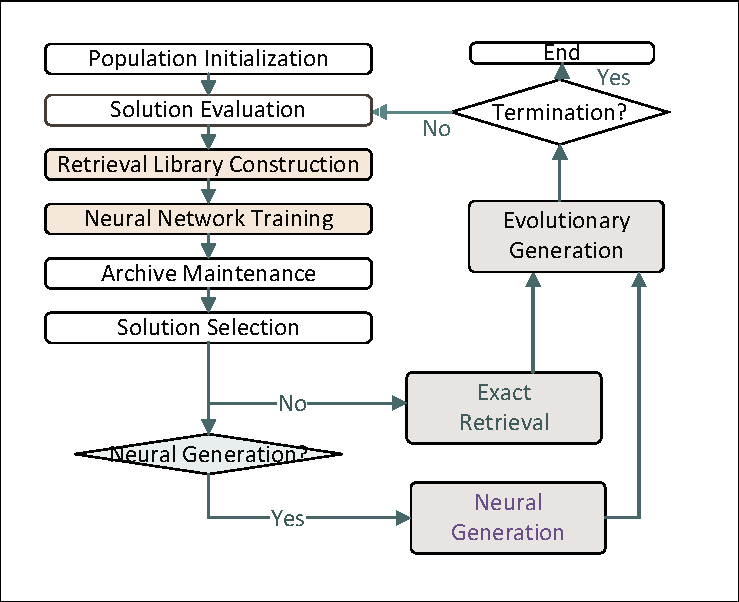
\includegraphics[width=0.75\linewidth, trim=10 15 10 15, clip]{figs/Flow.pdf}
                        \caption{The workflow of RAG-SR.}
                    \end{figure}

                    \textbf{\hlblue{Evolutionary algorithm with online learning:}}
                    \begin{enumerate}
                        \item \textbf{Solution Initialization:} Random initialization
                        \item \textbf{Solution Evaluation:} Ridge regression with leave-out cross-validation
                        \item \textbf{Library Construction:}
                        \begin{itemize}
                            \item \hlteal{Retrieval Library:} KD-Tree for nearest neighbor search
                            \item \hlpurple{Neural Library (Online learning):} Trained on Retrieval Library
                        \end{itemize}
                        \item \textbf{Solution Selection:} Lexicase selection
                        \item \textbf{Solution Generation:} Semantic Descent/Evolutionary operators
                        \item \textbf{Archive Maintenance:} Store best solutions
                    \end{enumerate}
                \end{block}

%----------------------------------------------------------------------------------------


            \end{column} % End of the first column

            \begin{column}{\sepwid}\end{column} % Empty spacer column

            \begin{column}{\onecolwid} % The second column

%----------------------------------------------------------------------------------------
%	SEMANTIC DESCENT
%----------------------------------------------------------------------------------------


                \begin{block}{Semantic Descent}
                    \textbf{\hlblue{For each tree $\phi_i$ in solution:}}
                    \begin{enumerate}
                        \item Remove contribution: $\Phi^{temp}(X) = \Phi(X) - \beta_i \phi_i(X)$
                        \item Compute residual: $R = Y - \Phi^{temp}(X)$
                        \item Generate new tree $\phi$ to fit $R$ using:
                        \begin{itemize}
                            \item \hlteal{Retrieval} with probability $1-P_{neural}$
                            \item \hlpurple{Neural generation} with probability $P_{neural}$
                        \end{itemize}
                        \item Accept new tree if it reduces error
                    \end{enumerate}
                \end{block}

%----------------------------------------------------------------------------------------
%	RETRIEVAL-AUGMENTED GENERATION
%----------------------------------------------------------------------------------------

                \begin{block}{Retrieval-Augmented Generation}
                    \begin{figure}
                        \centering
                        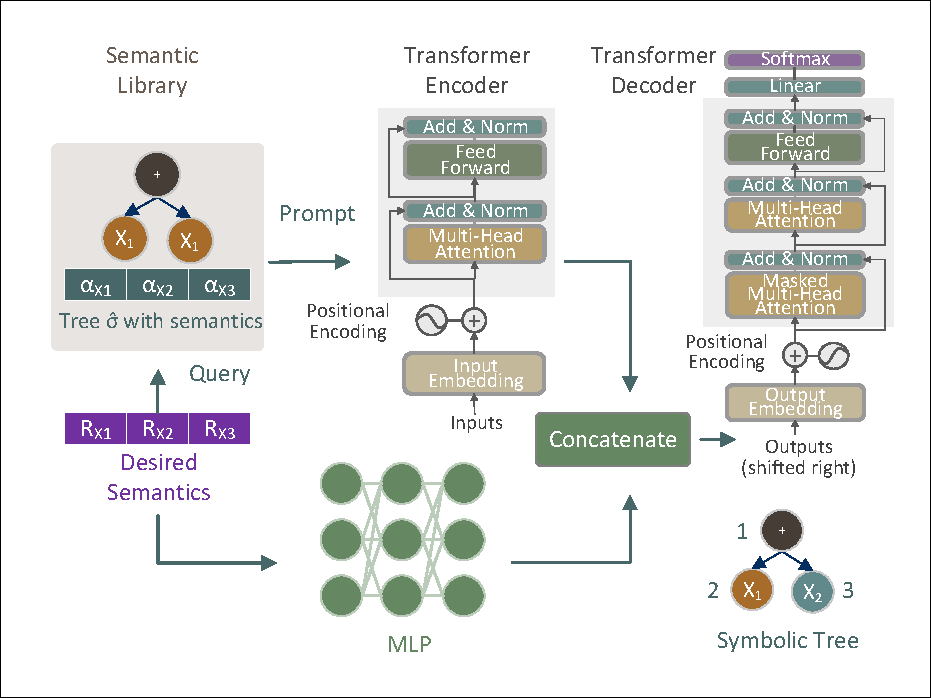
\includegraphics[width=\linewidth, trim=25 20 15 10, clip]{figs/Transformer.pdf}
                        \caption{Neural architecture for generating symbolic expressions.}
                    \end{figure}

                    \begin{itemize}
                        \item Masked Contrastive Learning for Semantically Equivalent Expressions
                        \item Scale-invariant Data Augmentation: Leverages sign-invariance
                        \item Double Query Strategy: Queries with both $R$ and $-R$
                    \end{itemize}
                \end{block}
                \vspace{-0.3cm}
                \begin{alertblock}{Key Takeaway}
                    \begin{center}
                        \textbf{\hlmodern{Language Model} $\rightarrow$ \hlmodern{Effective knowledge processing}}\\
                        \textbf{\hlmodern{Evolutionary Algorithm} $\rightarrow$ \hlmodern{Efficient knowledge discovery}}\\
                        \textbf{\hlmodern{RAG bridges LM and EA} $\rightarrow$ \hlmodern{Powerful SR}}
                    \end{center}
                \end{alertblock}
            \end{column} % End of the second column

            \begin{column}{\sepwid}\end{column} % Empty spacer column

            \begin{column}{\onecolwid} % The third column

%----------------------------------------------------------------------------------------
%	COMPONENT EVALUATION
%----------------------------------------------------------------------------------------


                \begin{block}{Key Results}
                    \begin{table}
                        \centering
                        \small
                        \begin{tabular}{cc}
                            \toprule
                            \textbf{\hlpurple{RAG-NN Generated}} & \textbf{\hlsteel{Simple NN Generated}} \\
                            \midrule
                            Sin(Sin(ARG3)) (0)                   & Cos(Cos(Cos(ARG9))) (4)                \\
                            AQ(ARG7, ARG8) (0)                   & Log(Max(ARG7, ARG7)) (3)               \\
                            Max(ARG1, ARG8) (0)                  & Subtract(ARG1, ARG1) (2)               \\
                            \bottomrule
                        \end{tabular}
                        \caption{Examples of generated trees with edit distance.}
                    \end{table}
                    \vspace{-5mm}

                    \begin{figure}
                        \centering
                        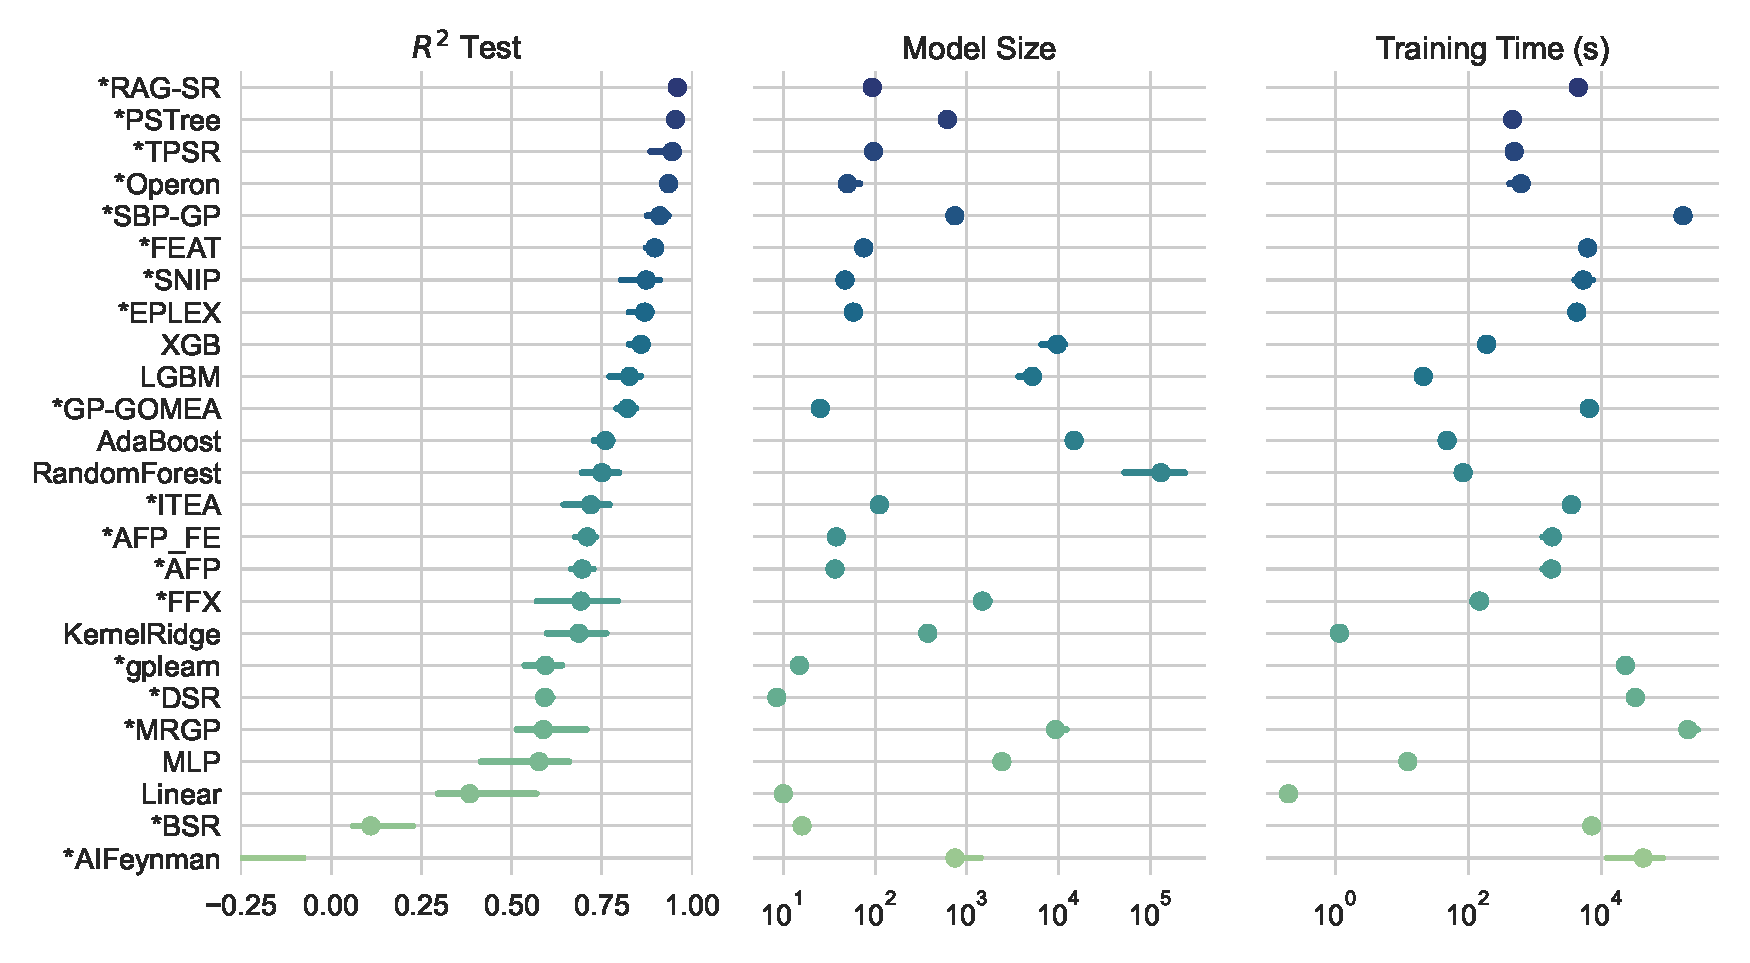
\includegraphics[width=\linewidth, trim=5 5 5 5, clip]{figs/pairgrid-pointplot_r2_test_model_size_training-time-(s).eps}
                        \caption{Comparison of test $R^2$ score, model size, and training time across 25 algorithms.}
                    \end{figure}


                    \begin{minipage}[t]{0.48\linewidth}
                        \begin{figure}
                            \centering
                            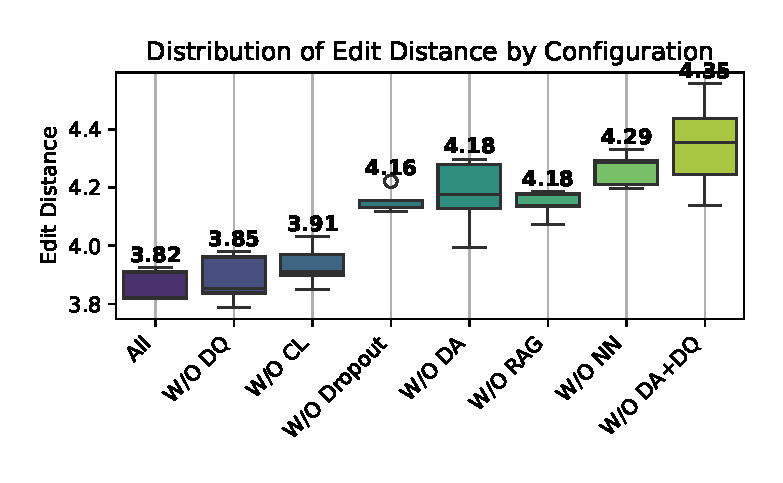
\includegraphics[width=\linewidth]{figs/ablation_study_accuracy_10.eps}
                            \caption{Edit distance under different configurations.}
                        \end{figure}
                    \end{minipage}
                    \hfill
                    \begin{minipage}[t]{0.48\linewidth}
                        \vspace*{.5cm} % Adjusted to align with figure
                        \textbf{\hlblue{Key Findings:}}
                        \begin{itemize}
                            \item \hlpurple{Neural generation outperforms simple retrieval}
                            \item \hlcharred{All components together achieve lowest edit distance, RAG has most significant impact}
                            \item \hlorange{RAG-SR outperforms all 25 algorithms in $R^2$ scores}
                        \end{itemize}
                    \end{minipage}

                    \vspace{45mm}

                    \begin{center}
                        \begin{tabular}{ccc}
                            % First column: QR code
                            \parbox[c][3.5in][c]{0.3\linewidth}{
                                
\includegraphics[width=\linewidth]{figs/QR.png}
                            }
                            \hspace{0.03\linewidth}
                            % Second column: AI Center and VUW-W logos
                            \parbox[c][3.5in][c]{0.3\linewidth}{
                                \vspace{8mm}
                                
\includegraphics[width=\linewidth]{figs/AI_Center.png}\\[1ex]
                                
\includegraphics[width=\linewidth]{figs/VUW-W.png}
                            }
                            \hspace{0.03\linewidth}
                            % Third column: MSU and ICLR logos
                            \parbox[c][3.5in][c]{0.3\linewidth}{
                                
\includegraphics[width=\linewidth]{figs/MSU.png}\\[1ex]
                                
\includegraphics[width=\linewidth]{figs/ICLR-logo.png}
                            }
                        \end{tabular}
                    \end{center}

%                    \begin{itemize}
%                        \item Effective online learning-based Symbolic Regression
%                        \item Retrieval augmentation that mitigates hallucination
%                    \end{itemize}
                \end{block}

%----------------------------------------------------------------------------------------
%	CONCLUSION
%----------------------------------------------------------------------------------------


%----------------------------------------------------------------------------------------


            \end{column} % End of the third column

            \begin{column}{\sepwid}\end{column} % Empty spacer column

        \end{columns} % End of all the columns in the poster

    \end{frame} % End of the enclosing frame

\end{document}

